\chapter{ARSITEKTUR \& DESAIN SISTEM}

\section{Arsitektur Teknologi}
Platform \textit{e-Learning} PT. BPR Jatim dibangun menggunakan arsitektur \textit{client-server} modern berbasis \textit{cloud} yang memisahkan lapisan tampilan klien (\textit{frontend}) dengan lapisan layanan dan basis data di server (\textit{backend}). Arsitektur ini dirancang untuk mewujudkan sistem yang \textit{scalable}, ringan, dan mudah dipelihara. Gambar \ref{fig:arsitektur} mengilustrasikan arsitektur teknologi sistem secara keseluruhan.

\begin{figure}[H]
    \centering
    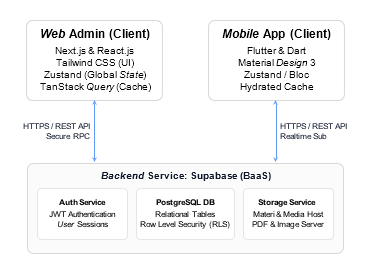
\includegraphics[width=0.9\textwidth]{image/insight-system-architecture.png}
    \caption{Arsitektur Teknologi Platform e-Learning PT. BPR Jatim}
    \label{fig:arsitektur}
\end{figure}

Pembagian peran teknologi pada arsitektur sistem adalah sebagai berikut:

\begin{table}[H]
\caption{Teknologi yang Digunakan dalam Platform e-Learning}
\label{tab:teknologi}
\centering
\begin{tabular}{|p{1cm}|p{3.5cm}|p{3cm}|p{7cm}|}
\hline
\textbf{No} & \textbf{Komponen} & \textbf{Teknologi} & \textbf{Deskripsi} \\ \hline
1 & Frontend Web Admin & Next.js (React) & Portal administrator yang di-\textit{deploy} di server \textit{hosting} internal / \textit{cloud} perusahaan untuk kemudahan akses. \\ \hline
2 & Frontend Mobile & Flutter SDK & Menghasilkan aplikasi Android (.apk) dan iOS (.ipa) berkinerja tinggi dari satu basis kode tunggal. \\ \hline
3 & Backend \& Database & Supabase Cloud & Menyediakan database relasional PostgreSQL, Supabase Auth untuk manajemen sesi login aman, dan Supabase Storage untuk menampung file PDF modul pelatihan. \\ \hline
\end{tabular}
\end{table}

\section{Use Case Diagram}
\textit{Use Case Diagram} pada Gambar \ref{fig:usecase} memetakan interaksi fungsional antara dua aktor utama (Karyawan dan Admin PSDM) dengan sistem. Diagram ini mendeskripsikan secara jelas batas hak akses dan cakupan fitur yang dapat dieksekusi oleh masing-masing aktor.

\begin{figure}[H]
    \centering
    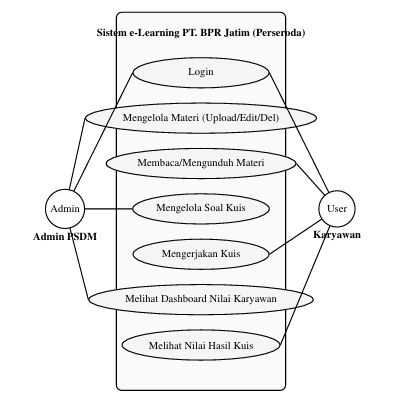
\includegraphics[width=0.75\textwidth]{image/usecase.png}
    \caption{Use Case Diagram Platform e-Learning}
    \label{fig:usecase}
\end{figure}

Berdasarkan diagram di atas, Admin PSDM memiliki hak akses untuk mengelola data karyawan, mengunggah modul pelatihan, membuat soal kuis, serta memantau rekapitulasi nilai. Sementara itu, Karyawan dapat mengakses materi pelatihan, mengerjakan kuis evaluasi, dan melihat riwayat nilai pribadinya.

\section{Flowchart Alur Bisnis Sistem}
Alur kerja sistem \textit{e-Learning} dari proses masuk (\textit{login}) hingga perekaman skor ujian digambarkan pada \textit{flowchart} berikut:

\begin{figure}[H]
    \centering
    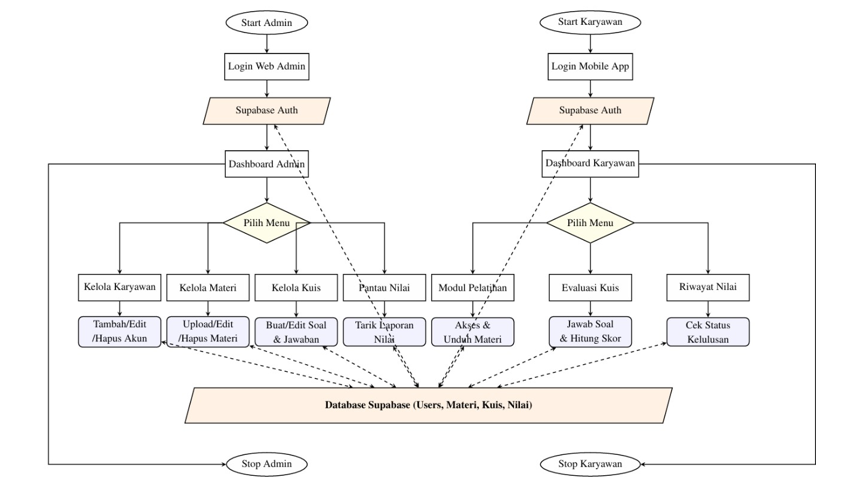
\includegraphics[width=\textwidth]{image/flowchart.png}
    \caption{Flowchart Alur Bisnis Platform e-Learning PT. BPR Jatim}
    \label{fig:flowchart_elearning}
\end{figure}

\section{Skema Basis Data (Entity Relationship Diagram)}
Skema basis data pada Gambar \ref{fig:erd} menggambarkan struktur tabel, atribut, serta relasi antartabel pada database relasional PostgreSQL yang dikelola melalui Supabase. Desain ERD ini dirancang untuk menjamin integritas rekam jejak pelatihan seluruh karyawan.

\begin{figure}[H]
    \centering
    
\includegraphics[width=0.85\textwidth]{image/erd-supabase.png}
    \caption{Entity Relationship Diagram (ERD) Basis Data e-Learning}
    \label{fig:erd}
\end{figure}

Database relasional PostgreSQL pada Supabase menggunakan tabel-tabel utama yang dijelaskan pada Tabel \ref{tab:database}.

\begin{table}[H]
\caption{Deskripsi Tabel Basis Data Platform e-Learning}
\label{tab:database}
\centering
\begin{tabular}{|p{0.8cm}|p{2.5cm}|p{11cm}|}
\hline
\textbf{No} & \textbf{Nama Tabel} & \textbf{Deskripsi} \\ \hline
1 & \texttt{users} & Menyimpan NIP, email, nama lengkap, role (admin/employee), dan ID divisi karyawan. \\ \hline
2 & \texttt{divisions} & Menyimpan ID divisi dan nama divisi (misal: Divisi TI, Operasional, PSDM). \\ \hline
3 & \texttt{modules} & Menyimpan judul modul, file path PDF modul di Supabase Storage, dan status ketersediaan pembelajaran. \\ \hline
4 & \texttt{exams} & Menyimpan judul ujian, batas waktu pengerjaan, Kriteria Ketuntasan Minimal (KKM), dan ID modul terkait. \\ \hline
5 & \texttt{questions} & Menyimpan detail butir soal kuis, pilihan ganda A/B/C/D, dan kunci jawaban benar. \\ \hline
6 & \texttt{results} & Menyimpan skor akhir, status kelulusan (Lulus/Gagal), dan tanggal pengerjaan kuis oleh karyawan. \\ \hline
\end{tabular}
\end{table}

\section{Keamanan Sistem}
Keamanan data merupakan aspek krusial dalam sistem \textit{e-Learning} di sektor perbankan. Platform ini mengimplementasikan beberapa lapisan keamanan sebagai berikut:

\begin{enumerate}
    \item \textbf{Autentikasi Berbasis Token JWT:} Setiap sesi login dikelola oleh Supabase Auth yang menghasilkan \textit{JSON Web Token} (JWT) \cite{jwt_security}. Token ini memiliki batas waktu kedaluwarsa (\textit{expiry time}) dan harus disisipkan pada setiap \textit{request} API untuk memvalidasi identitas pengguna.
    \item \textbf{Row Level Security (RLS):} Kebijakan keamanan tingkat baris diaktifkan pada seluruh tabel basis data. Melalui RLS, tiap karyawan hanya memiliki izin untuk melihat dan memproses rekam jejak nilainya sendiri, sementara Admin PSDM memiliki otorisasi penuh atas seluruh data.
    \item \textbf{Enkripsi Password:} Seluruh kata sandi pengguna dienkripsi menggunakan algoritma \textit{bcrypt} sebelum disimpan ke basis data, sehingga data kredensial tidak tersimpan dalam bentuk teks biasa (\textit{plain text}).
    \item \textbf{HTTPS \& SSL/TLS:} Seluruh komunikasi antara aplikasi klien dan server Supabase dilakukan melalui protokol HTTPS yang terenkripsi untuk mencegah penyadapan data (\textit{man-in-the-middle attack}).
\end{enumerate}
